\section{Introduction}
\label{sec:introduction}

% state the learning objective 

\hspace{0,5cm} This report is being made for the subject of Circuit Theory and Electronics Fundamentals and is related to the $2^{st}$ laboratory being its objective to study an RC circuit containing seven resistors (from $R_1$ to $R_7$), one sinusoidal voltage source ($v_s$), one capacitor ($C$), one current controlled voltage ($V_d$) source and one voltage controlled current source ($I_b$). The four elementary meshes are named after the current to which they are attributed, and the nodes are named after the numbers attributed to them, being $V_0$ the ground node.

The current controlled voltage source $V_d$ is calculated by multiplying $K_d$ with the current $I_d$, whereas the voltage controlled current source $I_b$ can be determined by multiplying $K_b$ with the voltage source $V_b$.

The display of this circuit, as well as the equations used to determine the value of $v_s$, can be seen in Figure~\ref{fig:circuito}.

In Section~\ref{sec:analysis} the circuit will be analysed theoretically with the aid of Octave, analysing firstly the circuit for $t<0$ using the nodal method, calculating the equivalent resistence $R_eq$ as seen from the capacitor terminals, determining the natural and forced solution for $V_6$ with the previous results, and finishing with the calculation of the frequency response for $V_c$, $V_s$ and $V_6$ and the study of these results.

Secondly, in Section~\ref{sec:simulation} it will be simulated the circuit using ngspice, with the aim of validating the results previously obtained by doing operating point, transient and frequency analysis.

Following with both results from Section~\ref{sec:analysis} and Section~\ref{sec:simulation} being compared and commented in Section ~\ref{sec:comparison}

The conclusions of this study are outlined in Section~\ref{sec:conclusion}.

\begin{figure}[H] \centering
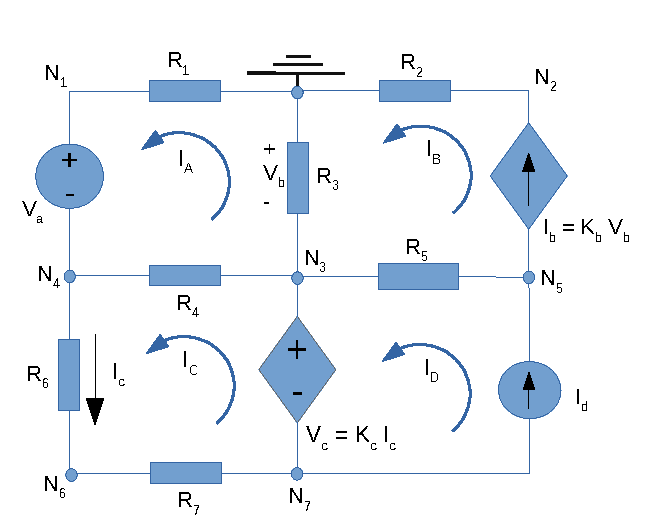
\includegraphics[width=1\linewidth]{circuito.pdf}
\caption{Circuit in analysis}
\label{fig:circuito}
\end{figure}


\newpage

Where:
\begin{center}
\begin{table}[H]
 \centering
  \begin{tabular}{|c|c|}
    \hline    
    {\bf Name} & {\bf Value [A or V]} \\ \hline
    \input{../mat/data_tab}
  \end{tabular}
  \caption{Results obtained by mesh analysis method with octave}
  \label{tab:mesh}
\end{table}
\end{center}

The units of the elements whose name starts with $R$ (the resistors) are $\Omega$ (ohm), $V_s$ is expressed in $V$ (volts) and $C$ is given in $F$ (farad). While $K_b$ is given in $S$ (siemens), $K_c$ is also given in $\Omega$.

These values where obtained using the Python script using the lowest student number on our group - 95785.


